\documentclass[a4paper]{article}
\usepackage[utf8]{inputenc}
\usepackage[english]{babel}

\usepackage{fullpage} % Package to use full page
\usepackage{parskip} % Package to tweak paragraph skipping
\usepackage{tikz} % Package for drawing
\usepackage{amsmath}
\usepackage{hyperref}
\usepackage{graphicx}


\usepackage[backend=biber, style=ieee]{biblatex}
\addbibresource{bibliography.bib} 

\title{Local Feature Matching}
\author{Ibrahim Onur Serbetci}
\date{16/02/2021}


\begin{document}

\maketitle
\section{Introduction}

Images can be matched by their features. These features can be often described with specific locations such as peaks, corners, edges. Therefore, the features can be used for matching these features from different images. In this report, these features have called corner points. Local feature matching pipeline consists of three main steps which are interest point detection, feature description and feature matching.

% PART 1
\section{Interest Point Detection}
For detecting interesting point two algorithm has implemented:

\textbullet{} Harris Corner Detection

\textbullet{} Adaptive Non-Maximal Suppression (ANMS)

%1.1
\subsection{Harris Corner Detection}

Harris corner detector is a corner detection algorithm introduced by Chris Harris and Mike Stephens in 1988 \cite{harris1988combined}. The implemented algorithm uses the Sobel operator to convolve image beyond both x and y axes after applying grey and Gaussian filter on the image. In this context, the auto-correlation function given below used to ensure that the features detected are stable.

\begin{equation}
M=w\begin{bmatrix}I_x^2 & I_xI_y \\ I_xI_y & I_y^2\end{bmatrix}
\end{equation}

The determinant of the auto-correlation matrix has used to calculate the following cornerness function.

\begin{equation}
R=g(I_x^2)g(I^2_y)-[g(I_xI_y)]^2-\lambda[g(I_x^2)+g(I_y^2)]^2
\end{equation}

Thus, the algorithm filter the image with Gaussian filter to ensure avoiding from over-fitting. Then, uses Sobel operator to filter edges beyond x and y axes and filter them with Gaussian filter again. This will construct to auto-correlation matrix given as $M$. The algorithm also uses the constant $\lambda$ to account for offsets that generally lies between $ \lambda \in[0.04:0.06]$.

%1.2
\subsection{Adaptive Non-Maximal Suppression (ANMS)}

After the implementation of the Harris corner detector we have $R$ matrix which contains cornerness score pixel by pixel. The algorithm applies 3x3 local maximum filter to find local maximum and ignore other ones. In this context, other than local maximums are encoded as 0. After that, algorithm calculates non-zero mean of the local maximum values and ignore values that are lower with the same technique. The algorithm is calculates the adaptive radius for each corner candidates that has survived from previous steps.

\begin{equation}
    r_i= min_j|x_i-x_j| \; s.t. f(x_i) < f(x_j)c_{robust} \; f(x_j),x_j\in{I}
\end{equation}

where $x_j$ is the candidate corner point, $x_i$ is the other point that meets the criteria and $f$ is the function that returns cornerness score of a point \cite{brown2005multi}. After finding the radius of the each candidate, the algorithm sorts largest to smallest the corners according to their radius and takes from the top $n$.

% PART 2
\section{Local Feature Description}

\textbullet{} Scale invariant feature transform (SIFT)

\textbullet{} Adaptive Non-Maximal Suppression (ANMS)

\subsection{SIFT-like Feature Descriptor}

For local description of each corner point from previous section, we used a SIFT-like algorithm. Firstly, the algorithm applies Gaussian filter and Sobel filter on the image with the parameters; $ksize=(3,3)$, $\sigma = 0.5$. Then, calculates angles and magnitudes of each point with the following formulas.


\begin{equation}
    \theta_{x,y} = \tan^{-1}(I_y \div I_x),
\end{equation}
\begin{equation}
    m_{x,y} = \sqrt{I_x^2 + I_y^2}
\end{equation}

The algorithm creates patches from hyper-parameter called feature width. For each 4x4 pixels, algorithm has binned them into 8 bins. Each of these bins represent 45 degrees.

\begin{figure}[!htbp]
\begin{center}
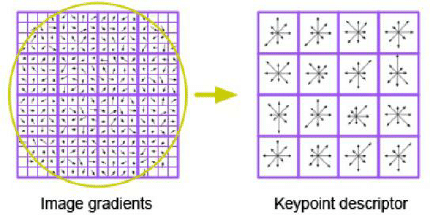
\includegraphics[width=6cm]{The-SIFT-descriptor-generation-2.png}
\end{center}
\caption{Illustration of histogram binning in SIFT \cite{sift}}
\label{sift_example}
\end{figure}

As it can be seen in the Figure \ref{sift_example}, we have $8*16=128$ values to describe each feature.



\subsection{SIFT with Multiple Scales}

While detecting interest points and describing them, multiple scales has been used. Image has resized with specific scales with several times. In this context the pipeline should be able to more adaptive to different scales of patches than one scaling. 

% PART 3
\section{Feature Matching with Nearest Neighbor Distance Ration (NNDR)}

The algorithm takes feature vectors and interest points' locations from previous steps. Finds the distance between each point's feature vector. Once it has all pair of the distance vector, it sorts ascending order and select the two features that has lowest distance. In order to pick best matches, algorithm limits the distances with certain threshold. The algorithm computes the ratio between two lowest distances and limits these ratios.


% RESULTS
\section{Results and Discussion}


Implementation of the Harris Corner Detector on the given 3 pair of images with the sigma parameter. The sigma parameters are; 3, 0.5 and 5 in order. The results of the implementation of Harris corner detector is in the Figure \ref{notre-harris}.

\begin{figure}[!htbp]
\begin{center}
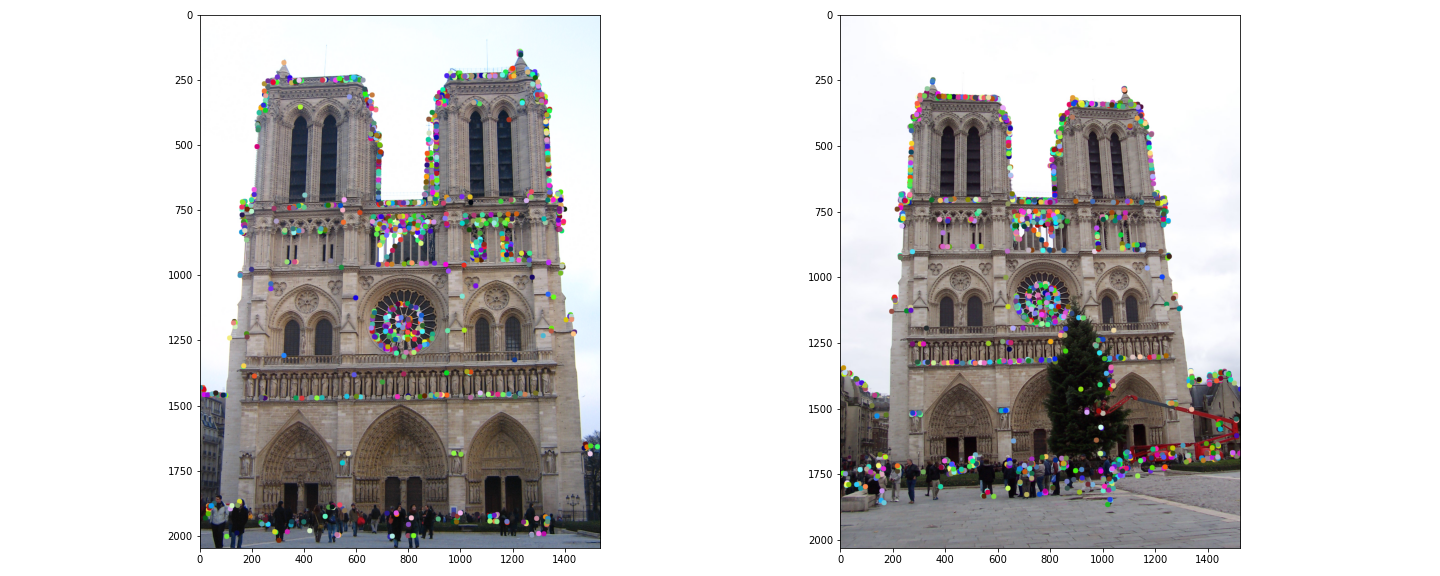
\includegraphics[width=10cm]{notre_dame_harris.png}
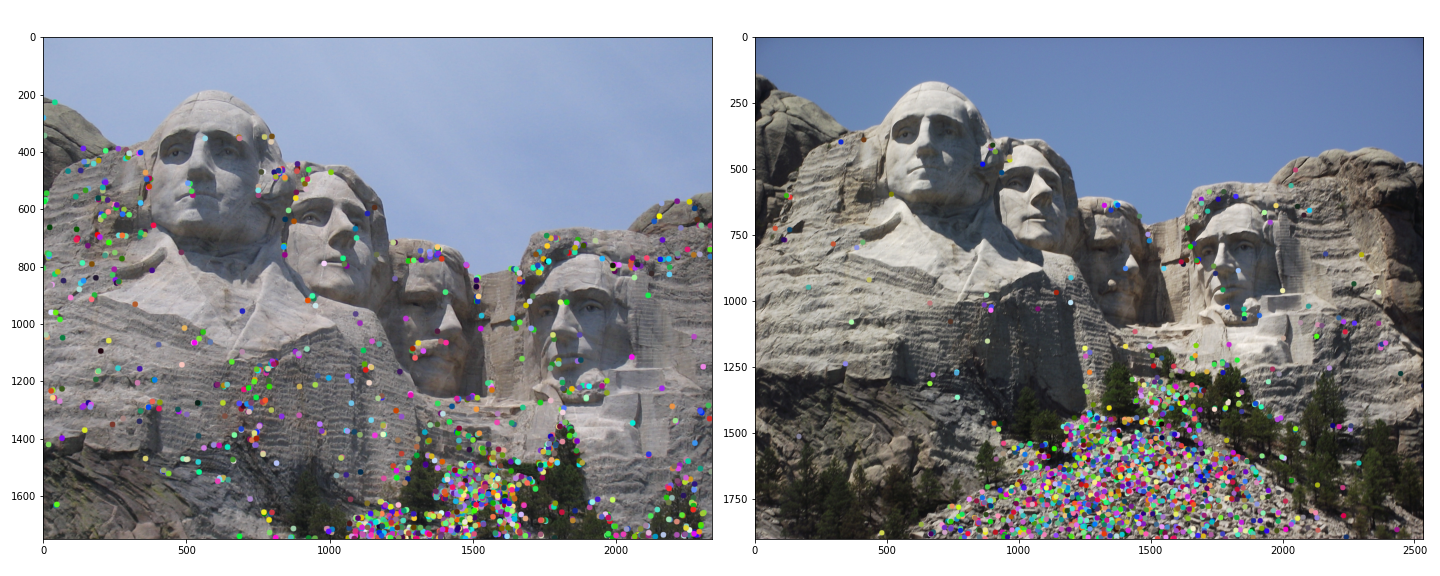
\includegraphics[width=8cm]{mt_rushmore_harris.png}
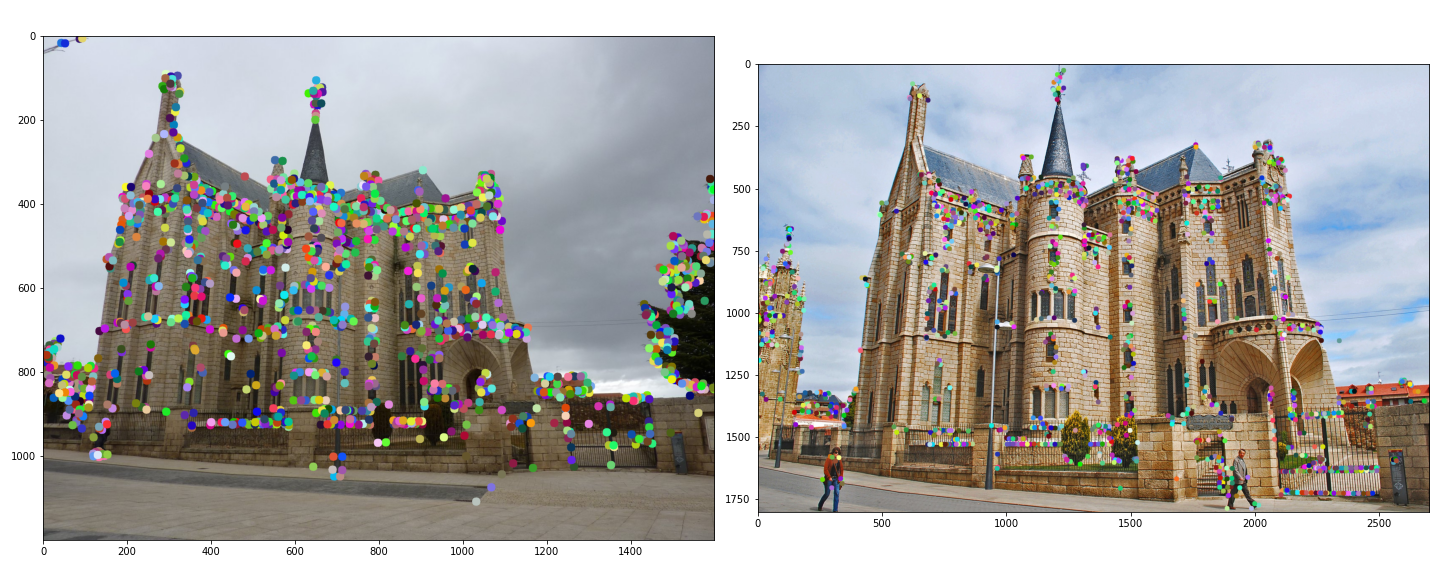
\includegraphics[width=8cm]{eg_harris.png}
\end{center}
\caption{Corners found with Harris Corner Detector and ANMS.}
\label{notre-harris}
\end{figure}


After implementing interest point detector algorithms, local feature descriptor can be implemented. The results from feature descriptor and matching functions provided in Table \ref{notre-table}.

\begin{table}[!htbp]
\centering
\begin{tabular}{||c c c c c c c c||} 
 \hline
 ID & Image & Feature Width & Sigma & Regularizer & Norm. Desc. & Cheat Pts. & Accuracy \\ [0.5ex] 
 \hline\hline
 1 & Notre Dame & 16 & 3 & No & No & No & 93\%\\ 
 2 & Notre Dame & 16 & 3 & No & Yes & No & 46\%  \\
 3 & Notre Dame & 16 & 3 & No & No & Yes & 78\%  \\
 4 & Mt. Rushmore & 44 & 0.5 & No & No & No & 99\% \\
 5 & Mt. Rushmore & 44 & 0.5 & No & Yes & No & 6\% \\
 6 & Mt. Rushmore & 44 & 0.5 & No & No & Yes & 62\% \\
 7 & Epis. Gaudi & 36 & 5 & Yes & No & No & 16\% \\ 
 8 & Epis. Gaudi & 36 & 5 & Yes & Yes & No & 5\% \\ 
 9 & Epis. Gaudi & 36 & 5 & Yes & No & Yes & 11\% \\  [1ex] 
 \hline
\end{tabular}
\caption{Result of pipeline implementation with different settings for top 100 matches.}\label{notre-table}
\end{table}

The local feature matching pipeline that we have implemented, has increased the accuracy score. As it can be seen in the Figure \ref{notre-table}, Notre Dame score has increased from 46\% to 93\%, Mountain Rushmore has increased from 6\% to 99\%, Episcopal Gaudi also has increased even from 5\% to 16\%. As an example, if we use SIFT-like self implemented method instead of Normalized Patches method for Notre Dame, accuracy score will be increased to 93\% from 78\%.

Sigma parameter is an important parameter to increase accuracy. The sigma parameter that has used for each image pair is different. The main purpose of the sigma is testing different blurring rate while applying Gaussian or any other filtering. The sigma represents standard deviation beyond x and y axes which means bigger sigma creates bigger blur in the image. Therefore, we can say that sigma one of the tools for regularization.

On the other hand, feature width parameter represents feature size of the image. Also length of the feature vector is calculated by feature width. Each image pair has used different feature width parameter which are 16, 36 and 44. It can be inferred from here that Mountain Rushmore images has needed to have bigger patch to create meaningful feature vector.

As it can be seen in the Table \ref{notre-table}, the best result has achieved with IDs: 1, 4, and 7. The most accurate matching occurred with Mt. Rushmore images - 99\%. The second accurate is the Notre Dame with 93\% accuracy score and the best result of the Episcopal Gaudi 16\%. Also, the visualization of the best results' can be seen in the Figure \ref{notre-result}.

\begin{figure}[!htbp]
\begin{center}
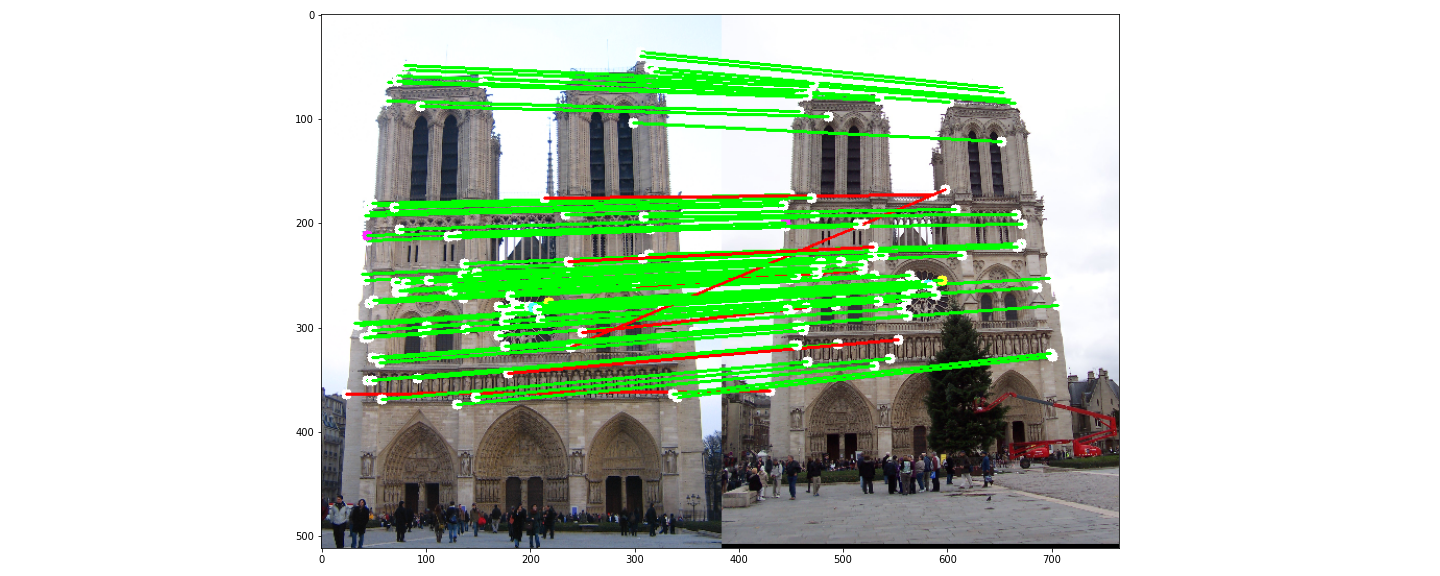
\includegraphics[width=12cm]{notre_dame.png}
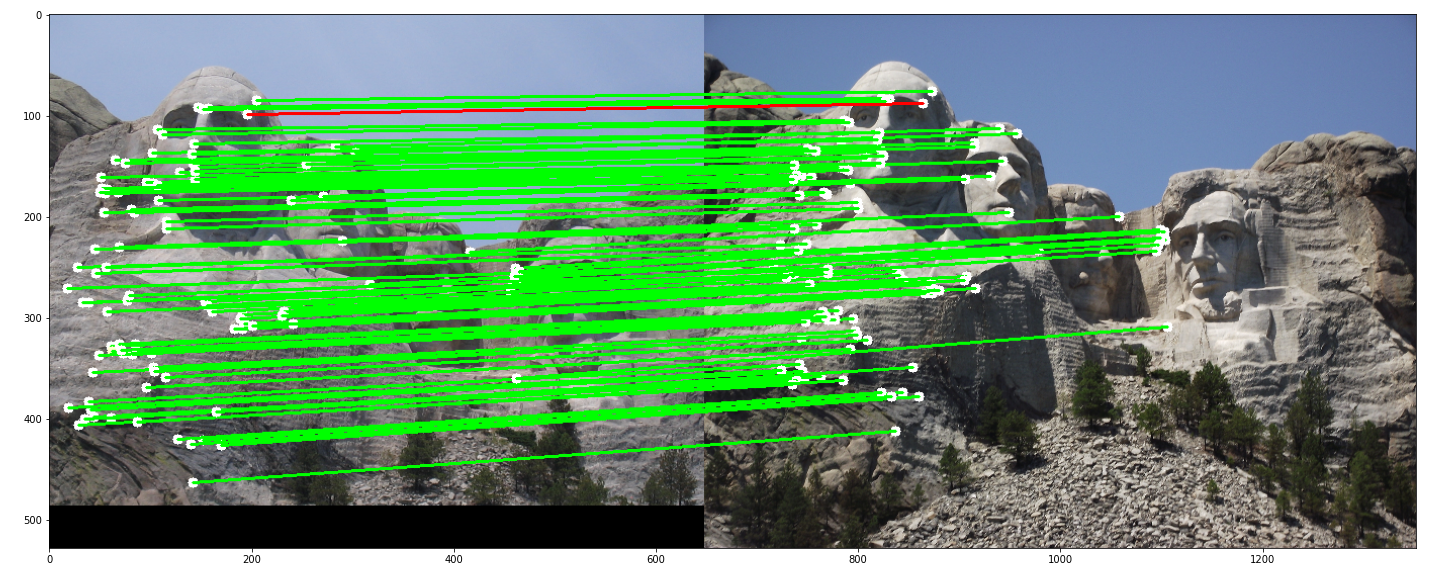
\includegraphics[width=10cm]{mt_rushmore.png}
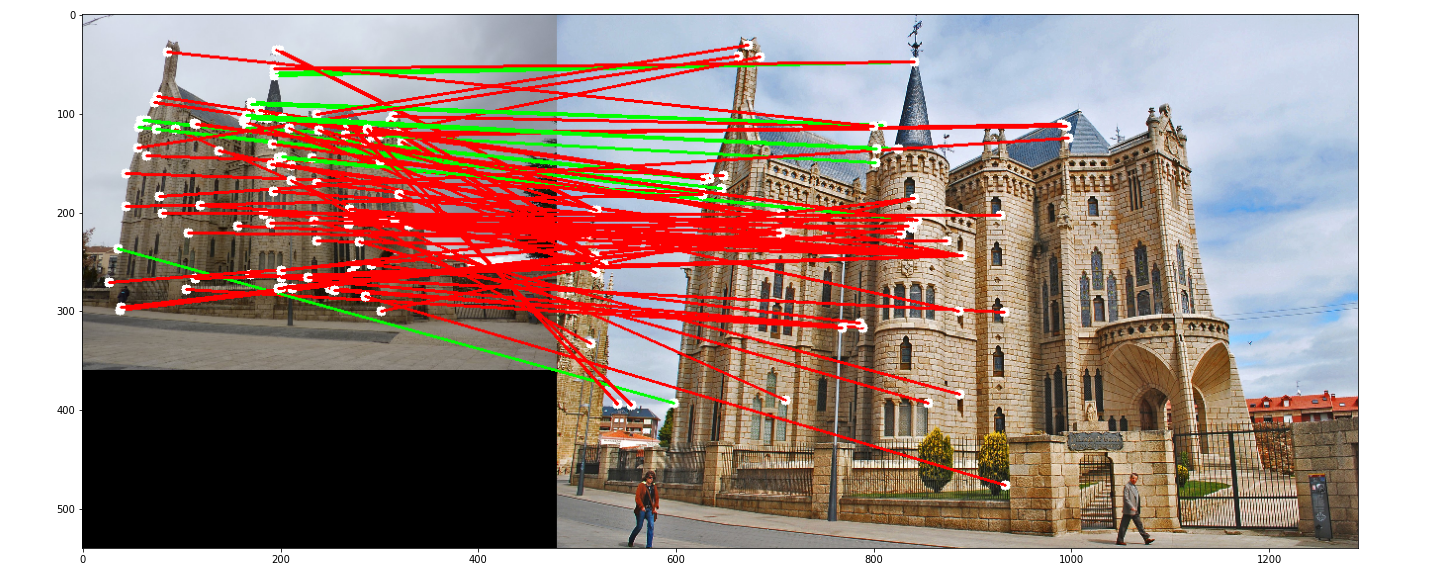
\includegraphics[width=10cm]{eg.png}
\end{center}
\caption{Visualization of the found best 100 matches for provided images.}
\label{notre-result}
\end{figure}

\printbibliography[title=References]
\end{document}